Figure~\ref{fig:eager_design} illustrates the main components of EAGER (in
blue) and their interactions. Solid arrows represent the interactions that take place
during application deployment-time, before an application has been validated
for deployment (an application may export zero or more web APIs). 
Short-dashed arrows represent deployment-time interactions that follow application validation.
Long-dashed arrows represent runtime interactions.

EAGER is invoked whenever a developer attempts to deploy an application, using
the developer tools available on his/her workstation. In some cloud
implementations these tools may be available as an online service accessed
via a web browser. In either case, the application deployment request is
intercepted by EAGER API Deployment Coordinator (ADC), which then performs the 
required governance checks based on the metadata stored in the Metadata Manager.
The Metadata Manager stores application names, versions, dependencies, API specifications,
user profiles and API keys.
Governance checks are driven by a set of administrator-specified policies that
are stored along with the ADC. These policy files are written in Python, and make use of 
the following assertion functions:

\begin{figure}
\centering
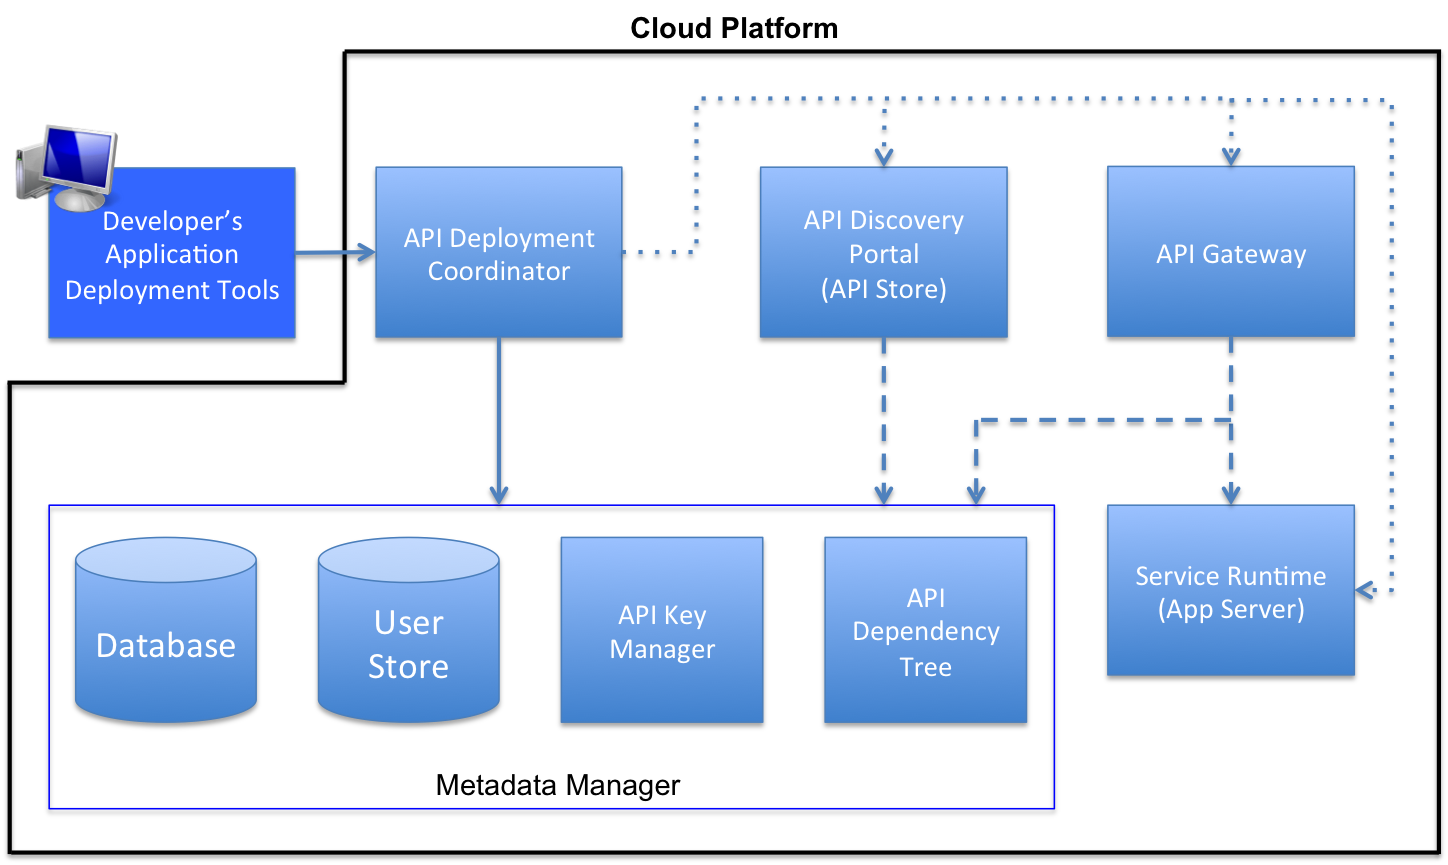
\includegraphics[scale=0.3]{eager_design}
\caption{EAGER Architecture}
\label{fig:eager_design}
\end{figure}

{\footnotesize 
\begin{lstlisting}[language=Python, frame=single]
assert_true(condition, optional_error_msg)
assert_false(condition, optional_error_msg)
assert_app_dependency(app, d_name, d_version)
assert_not_app_dependency(app, d_name, d_version)
assert_app_dependency_in_range(app, name,\
  lower, upper, exclude_lower, exclude_upper)
\end{lstlisting}
}

In order to keep all policy executions simple and stateless, EAGER prevents
policy code from accessing the file system, network and most third-party Python
libraries. Moreover, the policy language prohibits storoage of global state.

If a governance check fails (i.e. assertion failure), EAGER preempts the 
deployment process and returns an error. Otherwise it proceeds with the application deployment by
activating the deployment mechanisms on the developer's or administrator's
behalf. Additionally, all application metadata is saved to the Metadata Manager, and
if the application contains any web APIs, they will be published to the API Discovery Portal
and the API Gateway components. The API Discovery Portal is a web GUI that enables 
application developers to browse and
discover available APIs, and obtain the necessary API keys. The API Gateway intercepts
API calls at runtime and performs security, rate-limiting, and runtime policy checks . %In the future, we intend
%to use the API Gateway as a starting point to implement more comprehensive runtime
%API governance for cloud platforms.

In addition to the governance policy validations, EAGER also performs a set of built-in
sanity checks on all applications and APIs deployed in the PaaS cloud. One of these checks
is the backwards compatibility check. If EAGER detects that an API which is already deployed in
the cloud is being redeployed, it performs a comparison between the old
and latest specifications of the API to make sure that the developer is not introducing a backward
incompatible change to the API. This comparison is based on our past and ongoing work related
to syntactic and semantic similarity of web APIs~\cite{6930607}.

We implemented a prototype of EAGER using the AppScale open source PaaS cloud.  Prototype
was mostly implemented in Python, while using MySQL as the underlying datastore of the 
Metadata Manager. The prototype implementation did not require any code changes at the AppScale core.
However, we made configuration changes so that AppScale treats
EAGER components as built-in elements of the PaaS cloud.  As such, we 
are able to leverage the existing reliability and high availability mechanisms of AppScale to make 
EAGER components more reliable and high available. We also made some minor code modifications to the
AppScale developer tools, so that when a developer attempts to deploy an application into AppScale,
the deployment request is routed to the EAGER ADC.
